\section{Big-Step \ce} \label{sec:calc}

This section shows how the shared environment approach can be applied to
call-by-need evaluation. It starts with a big step semantics that abstracts away
environment representation, Curien's calculus of closures, and then shows how it
can be modified to force sharing. See Curien's call-by-name calculus of closures
in Figure~\ref{fig:curien}. \footnote{Curien calls it a ``lazy'' evaluator, and
there is some ambiguity with the term lazy, but here the term is used only to
mean call-by-need. Curien's condition checking that $i < m$ is omitted as the
semantics is only defined for closed terms.}

The App rule pushes a closure onto the environment, and the Id rule indexes into
the environment, entering the corresponding closure. This section shows that by
removing ambiguity about how the environments are represented, and forcing them
to be represented in a \emph{cactus stack}~\cite{stenstrom1988vlsi}, we can
define a novel call-by-need big step semantics.

To start, consider again the example from Section~\ref{sec:env}, this time with
de Bruijn indices: $(\lambda(\lambda t_0) \; (\lambda t_1)) t_2$.  The terms $t_0$
and $t_1$, when evaluated in Curien's calculus of closures, would have the
following environments, respectively: 

\begin{center}
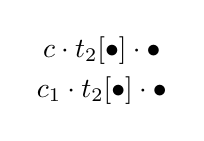
\begin{tikzpicture}
\node {$c \cdot t_2[\bullet] \cdot \bullet$};
\node [yshift=-0.5cm] {$c_1 \cdot t_2[\bullet] \cdot \bullet$};
\end{tikzpicture}
\end{center}

Again, the second closure is identical in each environment.  And again,
we can represent these environments with a shared environment, this time
keeping call-by-need evaluation in mind:
\begin{center}
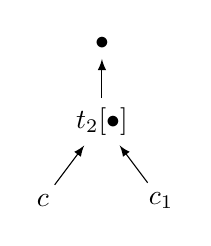
\begin{tikzpicture}[ 
  edge from parent path={(\tikzchildnode\tikzchildanchor) edge [-latex] (\tikzparentnode\tikzparentanchor)},
  level distance=1cm
]
\node (a) {$\bullet$} child{node (d) {$t_2[\bullet]$} child{node (b) {$c$}} child{node (c)
{$c_1$}}};

%\draw let \p1=(a), \p2 =(b), \n1={atan2(\y2-\y1,\x2-\x1)}, \n2={veclen(\y2-\y1,\x2-\x1)}
%  in ($ (a)!0.5!(b) $) ellipse [x radius=\n2/2+10pt, y radius=10pt, rotate=90-\n1];
%\draw let \p1=(a), \p2 =(c), \n1={atan2(\y2-\y1,\x2-\x1)}, \n2={veclen(\y2-\y1,\x2-\x1)}
%  in ($ (a)!0.5!(c) $) ellipse [x radius=\n2/2+10pt, y radius=10pt, rotate=90-\n1];
\end{tikzpicture}
\end{center}
This inverted tree structure seen earlier with the leaves pointing toward the
root is called a \emph{cactus stack} (sometimes called a spaghetti stack or
saguaro stack) when used to implement stacks~\cite{hauck1968burroughs,ichbiah1991rationale}, or a parent pointer tree in
general. In this use case, every node defines an environment as the sequence of
closures in the path to the root.  If $t_2[\bullet]$ is a thunk, and is updated
in place with the value after its first reference, then both environments would
contain the resulting value. This is exactly the kind of sharing that is
required by call-by-need, and thus we can use this structure to build a
call-by-need evaluator. This is the essence of the \ce machine. 

Curien's calculus of closures does not differentiate between flat and shared
environment representations; it has no need to. Therefore, we must derive a new
semantics, forcing the environment to be shared. Because we can hold the closure
directly in the environment, the standard approach of a heap of closures is
replaced with a \emph{heap of environments}. To enforce sharing, we extend
Curien's calculus of closures to explicitly include the heap of environments,
which we refer to as a \emph{cactus environment}. This is effectively a parent
pointer tree in which the contained objects are closures. 

See Figure~\ref{fig:bigstep} for the syntax and semantics of the \ce big step
semantics. Recall that we are only concerned with evaluation of closed terms.
The initial closed term $t$ is placed in a $(t[0],\epsilon[0 \mapsto \bullet])$
configuration, and evaluation terminates on a value. Some shorthand is used to
make heap notation more palatable for both the big-step semantics presented here
and the small step semantics presented in the next section. $\mu(l,i)=l' \mapsto
c \cdot l''$ denotes that looking up the $i$'th element in the linked
environment structure starting at $l$ results in location $l'$, where closure
$c$ and continuing environment $l''$ reside. $\mu(l) = c \cdot l'$ is the
statement that $l \mapsto c \cdot l' \in \mu$, and $\mu(u \mapsto c \cdot l')$
is $\mu$ with location $u$ updated to map to $c \cdot e$. Two 
different semantics are defined, one for call-by-name
(Figure~\ref{fig:bigstepname}) and one for call-by-need
(Figure~\ref{fig:bigstep}), which makes the connection to Curien's call-by-name
calculus more straightfoward. The rule for application is identical for both
semantics: each evaluates the left hand side to a function, then binds the
variable in the cactus environment, extending the current environment.

\begin{figure}
\textbf{Syntax}
\begin{align*}
\tag{Term} t &::= i \; | \; \lambda t \; | \; t \; t  \\
\tag{Variable} i &\in \mathbb{N}  \\
\tag{Closure} c &::= t \left[l\right] \\
\tag{Value} v &::= \lambda t \left[l\right] \\
\tag{Heap} \mu &::= \epsilon \; | \; \mu \left[ l \mapsto \rho \right] \\
\tag{Environment} \rho &::= \bullet \; | \; c \cdot l \\
\tag{Location} l,f &\in \mathbb{N}  \\
\tag{Configuration} s &::= \left(c, \mu \right)
\end{align*}
\textbf{Semantics}
\begin{align*}
\tag{Id} \inference
{\mu \left( l, i \right) = l' \mapsto c \cdot l'' \quad 
 \left(c, \mu\right) \Downarrow \left(v, \mu'\right)}
{\left(i\left[l\right],\mu\right) \Downarrow \left(v, \mu'\right)}
\end{align*} 
\begin{align*}
\tag{App} \inference
{\left(t\left[l\right], \mu\right) \Downarrow \left(\lambda t_2\left[l'\right], \mu'\right) 
   \quad f \not \in \textnormal{dom}\left(\mu'\right)
   \\ \left(t_2\left[f\right], \mu'\left[f \mapsto t_3\left[l\right] \cdot l'\right]\right)
         \Downarrow 
      \left(v, \mu'' \right) 
   }
{\left(t \; t_3\left[l\right], \mu\right) \Downarrow \left(v, \mu'' \right)}  
\end{align*} 
\begin{align*}
\tag{Abs} \inference {} {\left(\lambda t\left[l\right], \mu\right) \Downarrow \left(\lambda t\left[l\right], \mu\right)}
\end{align*}
\caption{Big-step call-by-name \ce syntax and semantics}
\label{fig:bigstepname}
\end{figure}


The only difference between this semantics and Curien's is that if we need
to extend an environment multiple times, the semantics \emph{requires}
sharing it among the extensions. This makes no difference for call-by-name, but
it is needed for the sharing of results in the Id rule. The explicit
environment sharing ensures that the closure that is overwritten with a
value is shared correctly.

\begin{figure}
\textbf{Syntax}
\begin{align*}
\tag{Term} t &::= i \; | \; \lambda t \; | \; t \; t  \\
\tag{Variable} i &\in \mathbb{N}  \\
\tag{Closure} c &::= t \left[l\right] \\
\tag{Value} v &::= \lambda t \left[l\right] \\
\tag{Heap} \mu &::= \epsilon \; | \; \mu \left[ l \mapsto \rho \right] \\
\tag{Environment} \rho &::= \bullet \; | \; c \cdot l \\
\tag{Location} l,f &\in \mathbb{N}  \\
\tag{Configuration} s &::= \left(c, \mu \right)
\end{align*}
\textbf{Semantics}
\begin{align*}
\tag{Id} \inference
{\mu \left( l, i \right) = l' \mapsto c \cdot l'' \quad 
 \left(c, \mu\right) \Downarrow \left(v, \mu'\right)}
{\left(i\left[l\right],\mu\right) \Downarrow \left(v, \mu'\left[l' \mapsto v \cdot l''\right]\right)}
\end{align*}
\begin{align*}
\tag{App} \inference
{\left(t\left[l\right], \mu\right) \Downarrow \left(\lambda t_2\left[l'\right], \mu'\right) 
   \quad f \not \in \textnormal{dom}\left(\mu'\right)
   \\ \left(t_2\left[f\right], \mu'\left[f \mapsto t_3\left[l\right] \cdot l'\right]\right)
         \Downarrow 
      \left(v, \mu'' \right) 
   }
{\left(t \; t_3\left[l\right], \mu\right) \Downarrow \left(v, \mu'' \right)}  
\end{align*}
\begin{align*}
\tag{Abs} \inference {} {\left(\lambda t\left[l\right], \mu\right) \Downarrow \left(\lambda t\left[l\right], \mu\right)}
\end{align*}
\caption{Big-step call-by-need \ce syntax and semantics}
\label{fig:bigstep}
\end{figure}

